\documentclass[11pt]{article}

% Change "review" to "final" to generate the final (sometimes called camera-ready) version.
% Change to "preprint" to generate a non-anonymous version with page numbers.
\usepackage[final]{acl}

% Standard package includes
\usepackage{times}
\usepackage{latexsym}

% For proper rendering and hyphenation of words containing Latin characters (including in bib files)
\usepackage[T1]{fontenc}
% For Vietnamese characters
% \usepackage[T5]{fontenc}
% See https://www.latex-project.org/help/documentation/encguide.pdf for other character sets

% This assumes your files are encoded as UTF8
\usepackage[utf8]{inputenc}

% This is not strictly necessary, and may be commented out,
% but it will improve the layout of the manuscript,
% and will typically save some space.
\usepackage{microtype}

% This is also not strictly necessary, and may be commented out.
% However, it will improve the aesthetics of text in
% the typewriter font.
\usepackage{inconsolata}

%Including images in your LaTeX document requires adding
%additional package(s)
\usepackage{graphicx}

\usepackage{float}
% \usepackage{multicol}

% If the title and author information does not fit in the area allocated, uncomment the following
%
%\setlength\titlebox{<dim>}
%
% and set <dim> to something 5cm or larger.

\title{SYNAPSE: Summarization \& Answering with Precision via Scalable Encoding}

\author{ Yajat Rangnekar \\
2023114008 \And
  Manas Mittal \\
2024121003\And
  George Rahul \\
2024121013}

\begin{document}
\maketitle

\begin{abstract}
Standard Transformer models are computationally expensive and cannot process long documents like books, legal texts, or in-depth reports in their entirety. This limits their use in comprehensive understanding tasks. We would like to design, build, and evaluate a hierarchical NLP system that can process arbitrarily long documents efficiently. The system will be capable of performing both high-level "gist" tasks (like summarization) and fine-grained "detail" tasks (like question answering) while maintaining factual consistency with the source text.
\end{abstract}

\section{Introduction}

The central idea of this project is to develop \textbf{SYNAPSE} (Summarization \& Answering with Precision via Scalable Encoding), a novel hierarchical framework designed to overcome the significant computational limitations of standard Transformer models when processing long-form documents. 

The current state-of-the-art architectures, while powerful, are constrained by a quadratic complexity in their self-attention mechanism, making them impractical for document-scale analysis \citep{vaswani2023attentionneed}. SYNAPSE addresses this ``quadratic bottleneck'' by adopting a multi-stage, ``divide-and-conquer'' approach that enables both high-level comprehension and fine-grained factual extraction within a single, unified system.

The proposed solution operates via a three-stage pipeline:
\begin{enumerate}
    \item \textbf{Scalable Encoding: }The system first ingests a long document and parses it into a sequence of smaller, semantically coherent text chunks. It then employs a Transformer-based Denoising Autoencoder to learn a dense and meaningful vector representation (embedding) for each chunk. This initial stage effectively compresses the long document into a computationally tractable sequence of high-information vectors.
    \item \textbf{Task-Adaptive Processing: }The core innovation of SYNAPSE lies in its dual-pathway approach to processing this sequence of embeddings:
    \begin{enumerate}
        \item For \textbf{Summarization}, which requires a global understanding of the document, the system leverages the entire sequence of chunk embeddings as a high-level abstractive representation.
        \item For \textbf{Answering with Precision}, where factual accuracy is paramount, the system implements an approach similar to Retrieval-Augmented Generation (RAG) \citep{lewis2021retrievalaugmentedgenerationknowledgeintensivenlp}. A user question is embedded and used to perform a rapid similarity search over the document's chunk embeddings. The system then retrieves the original raw text of the most relevant chunks, providing verifiable source material for the final answer.
    \end{enumerate}
    \item \textbf{Unified Text Generation: }A single generative model, built on a unified text-to-text framework like T5 \citep{raffel2023exploringlimitstransferlearning}, acts as the final output layer. It interprets task-specific prefixes, allowing it to fluidly switch between summarization and precise answering.
\end{enumerate}

By synthesizing these techniques, SYNAPSE aims to create a system that is both scalable for long documents and factually reliable. Its key contribution is a unified framework that provides broad summarization and precise answering, mitigating the risk of hallucinations by grounding responses directly in the source text.

\section{Related Works}

SYNAPSE builds upon several recent advances in representation learning and document processing:

\begin{enumerate}
    \item \textbf{Self-Attention and Long-Form Constraints:} Transformer-based models are effective but face quadratic complexity challenges when scaling to long sequences \citep{vaswani2023attentionneed}.
    \item \textbf{Unsupervised Representation Learning:} Our scalable encoding strategy draws inspiration from Transformer-based Denoising Autoencoders, which have demonstrated strong results in learning robust sentence and passage embeddings \citep{wang2021tsdaeusingtransformerbasedsequential}.
    \item \textbf{Retrieval-Augmented Generation:} The answering pathway aligns with the Retrieval-Augmented Generation paradigm, where retrieval enhances factual accuracy \citep{lewis2021retrievalaugmentedgenerationknowledgeintensivenlp}. SYNAPSE extends this concept by embedding retrieval within its architecture.
    \item \textbf{Unified Text-to-Text Frameworks:} Models like T5 have shown that a single generative framework can handle multiple NLP tasks by using task-specific prefixes \citep{raffel2023exploringlimitstransferlearning}.
\end{enumerate}

By integrating these approaches, SYNAPSE proposes a cohesive architecture that balances computational efficiency with factual accuracy for long-document summarization and question answering.


\section{Methodology}

The design of SYNAPSE follows a hierarchical, multi-stage pipeline that enables efficient handling of long documents while maintaining factual grounding in the source. The methodology can be divided into three primary stages: (i) scalable encoding of long texts, (ii) task-adaptive processing for summarization and question answering, and (iii) unified generation through a single sequence-to-sequence model.

\subsection{Stage 1: Scalable Encoding}
Long input documents are first segmented into semantically coherent chunks. Instead of relying only on fixed-length splits, we explore semantic segmentation techniques that aim to preserve coherence within each chunk. Specifically, we employ SBERT embeddings \citep{reimers2019sentencebertsentenceembeddingsusing} to represent individual sentences, and then apply similarity-based methods such as cosine similarity to cluster or group adjacent sentences. This allows us to divide the document into semantically meaningful segments rather than arbitrary spans. 

To further refine segmentation, we experiment with two design choices: (i) varying the chunk size to study the trade-off between context preservation and computational efficiency, and (ii) introducing overlaps between adjacent chunks to avoid boundary information loss.

Once the chunks are created, each is encoded into a dense representation. Our initial approach is to use a Transformer-based Denoising Autoencoder, trained to reconstruct masked or corrupted segments. The encoder component produces compact embeddings that capture the semantic meaning of each chunk while filtering out noise. In parallel, we also investigate an alternative design based on sequence-to-sequence models, where encoder hidden states are directly used as chunk embeddings. This dual strategy allows us to compare reconstruction-based embeddings with encoder-only representations and evaluate their downstream effectiveness.

\begin{figure}[H]
    \centering
    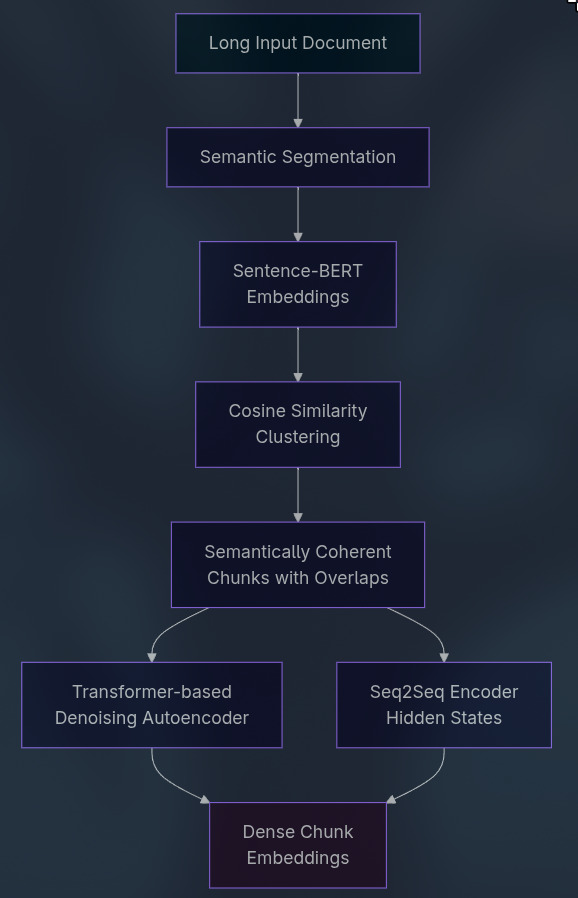
\includegraphics[width=0.6\columnwidth]{images/Stage_1.jpeg}
    \caption*{Stage 1: Scalable Encoding}
    \label{fig:stage1}
\end{figure}

\subsection{Stage 2: Task-Adaptive Processing}
Once embeddings are obtained, SYNAPSE dynamically determines the downstream processing pathway. This routing can be performed either through a simple rule-based mechanism (e.g., based on task prefix or query type) or through a lightweight binary classifier trained to decide whether the input corresponds to a summarization or question answering task.

\paragraph{Summarization Pathway.} For summarization, the system aggregates the chunk embeddings into a sequence that represents the entire document. This aggregated representation captures global dependencies across chunks and serves as input for high-level text generation.

\paragraph{Answering with Precision Pathway.} For question answering, the user query is first embedded into the same latent space as the document chunks. A similarity search retrieves the most relevant chunks, and their embeddings are combined with the query embedding to form a task-specific representation. This ensures factual grounding while keeping the input computationally tractable.

At the end of this stage, both summarization and QA tasks are represented uniformly as structured embeddings, ready for the unified generative model in Stage~3.

\begin{figure}[H]
    \centering
    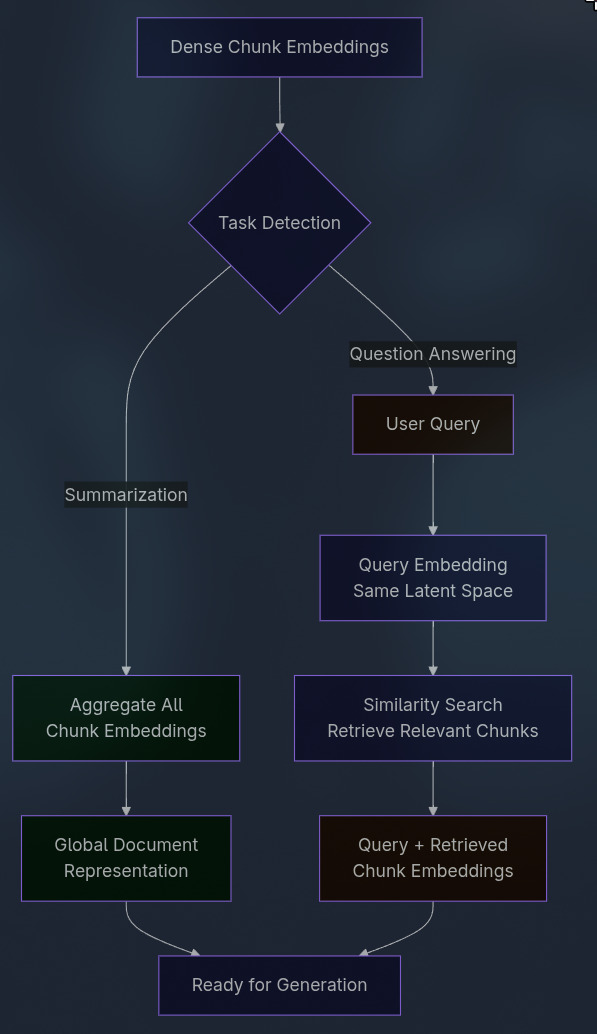
\includegraphics[width=0.6\columnwidth]{images/Stage_2.jpeg}
    \caption*{Stage 2: Task-Adaptive Processing}
    \label{fig:stage2}
\end{figure}

\subsection{Stage 3: Unified Text Generation}
The final stage of SYNAPSE is a unified generative model that produces natural language outputs for both summarization and question answering. We adopt a text-to-text Transformer architecture (e.g., T5 \citep{raffel2023exploringlimitstransferlearning}), extended to operate over embeddings rather than raw text. This ensures scalability to very long documents without exceeding token limits.

Task-specific prefixes  (e.g., \texttt{summarize:} or \texttt{answer:}) or the binary classifier/router guide the model to perform the appropriate task. For summarization, the generator conditions on the sequence of aggregated chunk embeddings; for QA, it conditions on the query embedding together with the retrieved chunk embeddings.

A central design question is how to transform embeddings into inputs suitable for the generator. We propose several ablation strategies:
\begin{enumerate}
    \item \textbf{Direct Decoding:} Train a decoder that consumes embeddings directly and generates text.
    \item \textbf{Adapter Layers:} Extend a pre-trained Transformer with adapters that learn to interpret embeddings as hidden-state inputs.
    \item \textbf{Embedding-to-Text Dictionary:} Use a learned dictionary that maps embeddings back to their corresponding text spans, combining retrieval-based evidence with generative flexibility.
\end{enumerate}

By consolidating both summarization and QA under a single backbone, SYNAPSE eliminates the need for task-specific models while ensuring consistent, scalable performance across tasks.

Through this modular yet unified methodology, SYNAPSE balances efficiency and accuracy: scalable encoding enables handling of arbitrarily long texts, retrieval ensures factual precision, and unified generation maintains flexibility across multiple tasks.

\begin{figure}[H]
    \centering
    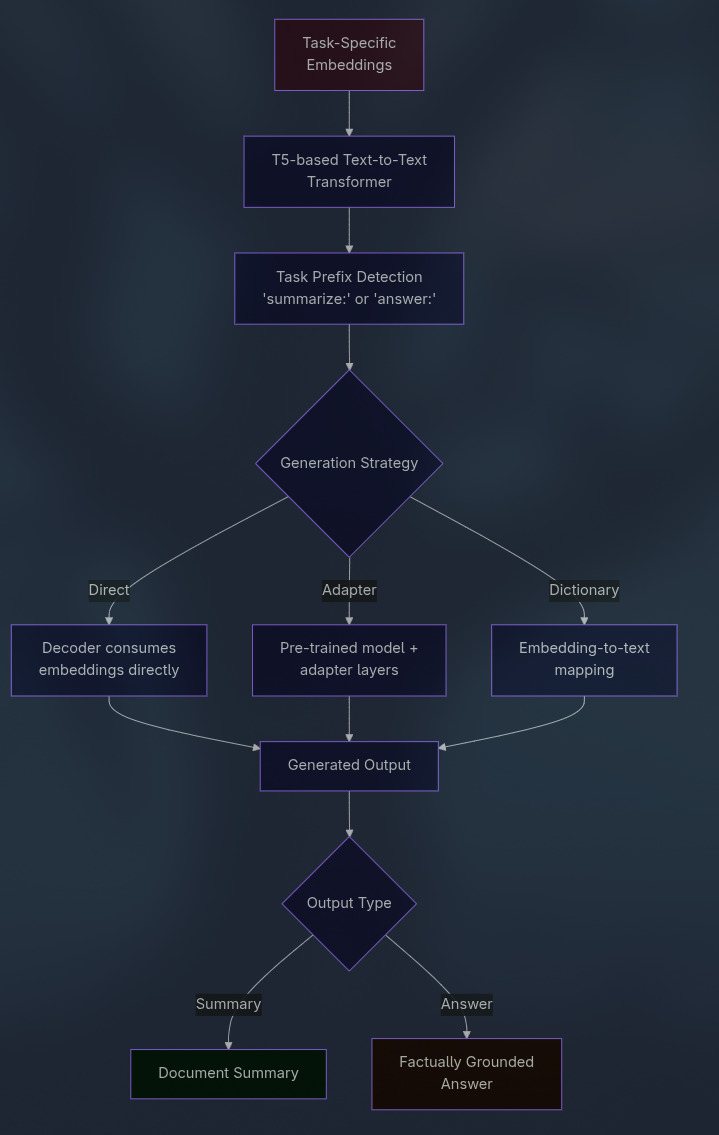
\includegraphics[width=0.6\columnwidth]{images/Stage_3.jpeg}
    \caption*{Stage 3: Unified Answering System}
    \label{fig:stage2}
\end{figure}

\section{Datasets}
For evaluating SYNAPSE, we focus on two datasets that are explicitly designed to test long-document comprehension and question answering. Both datasets require reasoning over extended contexts, making them suitable for validating our hierarchical encoding and retrieval-augmented answering framework.

\subsection{NarrativeQA}
NarrativeQA \citep{kočiský2017narrativeqareadingcomprehensionchallenge} is a reading comprehension dataset built from books and movie scripts (around 1,567 stories), paired with human-written summaries and question answer pairs (total of 46,765 pairs). The dataset provides two main evaluation settings: (i) \textit{Summaries Only}, where questions must be answered based on a Wikipedia-style summary of the narrative, and (ii) \textit{Stories Only}, which requires models to operate over the full long-form text, often tens of thousands of words in length. Because of its scale and narrative complexity, NarrativeQA forces models to perform chunk-based retrieval and deep comprehension across lengthy contexts, aligning directly with SYNAPSE's scalable encoding and hierarchical summarization design.

\subsection{PeerQA}
PeerQA \citep{baumgärtner2025peerqascientificquestionanswering} is a scientific question answering dataset derived from peer review comments and author responses. It consists of 579 question answer pairs covering 208 long academic papers, primarily in ML and NLP. Each reviewer comment acts as a question, and the corresponding author response serves as an answer grounded in the original paper. PeerQA supports three tasks: (i) evidence retrieval, (ii) unanswerable question detection, and (iii) answer generation. With documents averaging around 12,000 tokens, PeerQA presents significant computational challenges for conventional Transformer architectures. Its emphasis on factual precision and retrieval of supporting evidence makes it highly relevant for evaluating the retrieval-augmented answering pathway in SYNAPSE. Furthermore, by leveraging the abstracts of research papers as proxies for their summaries, we can design an additional evaluation setting that simultaneously exercises both core capabilities of SYNAPSE: long-document summarization and precise question answering.

\section{Evaluation}
To rigorously assess the performance of the SYNAPSE framework, we will employ a multi-faceted evaluation strategy that measures the quality of each component as well as the end-to-end performance on the primary tasks.

\subsection{Evaluating Representation Learning (The Autoencoder)}
The quality of the learned chunk embeddings is foundational to the entire system. We will evaluate it both intrinsically and extrinsically:
\begin{itemize}
    \item \textbf{Intrinsic Evaluation:} The primary metric for the autoencoder's training is its reconstruction loss \citep{michelucci2022introductionautoencoders}. A lower loss indicates that the latent embeddings are successfully capturing the essential information required to reconstruct the original text.
    \item \textbf{Extrinsic Evaluation:} The ultimate test of the embeddings is their performance on downstream tasks. The performance of the summarization and QA models will serve as the most meaningful validation of the representations' quality.
\end{itemize}

\subsection{Evaluating Summarization}
The quality of the generated summaries will be assessed using standard, widely-accepted metrics that measure lexical overlap and semantic similarity:
\begin{itemize}
    \item \textbf{ROUGE (Recall-Oriented Understudy for Gisting Evaluation)} \citep{lin-2004-rouge}: We will report F1 scores for ROUGE-1 (unigram overlap), ROUGE-2 (bigram overlap), and ROUGE-L (longest common subsequence), which measures structural similarity.
    \item \textbf{BERTScore} \citep{zhang2020bertscoreevaluatingtextgeneration}: To move beyond simple lexical overlap, we will use BERTScore, which computes a similarity score between tokens in the candidate and reference summaries using contextual embeddings. This provides a more robust measure of semantic equivalence.
\end{itemize}

\subsection{Evaluating Question Answering}
The Answering with Precision component will be evaluated on its factual accuracy and fluency:
\begin{itemize}
    \item \textbf{Standard QA Metrics:} We will use the standard metrics from the SQuAD benchmark \citep{rajpurkar2016squad100000questionsmachine}: Exact Match (EM), which measures the percentage of predictions that match the ground-truth answers exactly, and F1-Score, which measures the harmonic mean of precision and recall at the token level. These are excellent for measuring lexical accuracy.
    \item \textbf{Semantic Similarity Metrics:} Since our model is generative, its answers may be semantically correct but lexically different from the ground truth. Therefore, we will also report BERTScore to evaluate the semantic similarity between the generated answer and the reference answer.
    \item \textbf{Generation Metrics:} We may also report metrics like BLEU \citep{papineni-etal-2002-bleu}, which is traditionally used in machine translation but is also widely applied to measure the quality of text generation tasks.
\end{itemize}

\bibliography{custom}

\end{document}
